% !TEX root = thesis.tex
%%%%%%%%%%%%%%%%%%%%%%%%%%%%%%%%%%%%%%%%%%%%%%%%%%%%%%%%%%%%%%%%%%%%%%%%%%%%%%%%
\chapter{Разработка инструментальной среды}
%%%%%%%%%%%%%%%%%%%%%%%%%%%%%%%%%%%%%%%%%%%%%%%%%%%%%%%%%%%%%%%%%%%%%%%%%%%%%%%%

Разработка среды велась на языке Java 7 версии (OpenJDK Runtime Environment
(IcedTea 2.4.7)~\cite{Gosling2013}).

%%%%%%%%%%%%%%%%%%%%%%%%%%%%%%%%%%%%%%%%%%%%%%%%%%%%%%%%%%%%%%%%%%%%%%%%%%%%%%%%
\section{Структура проекта}
%%%%%%%%%%%%%%%%%%%%%%%%%%%%%%%%%%%%%%%%%%%%%%%%%%%%%%%%%%%%%%%%%%%%%%%%%%%%%%%%

В соответствии с архитектурой среды, приведенной в п.п.~\ref{sec:architecture},
проект разбит на 3 составляющих:

\begin{enumerate}
    \item Метамодель
    \item Преобразователи
    \item Инструментальная среда (графический интерфейс, процедуры визуализации
    и анализа)
\end{enumerate}

\nomenclature{POM}{Project Object Model, способ описания проекта в система
автоматизированной сборки Maven}

Сборка проекта производится при помощи фреймворка для автоматизации сборки
Apache Maven. Данный фреймворк позволяет декларативным образом описывать процесс
сборки проекта, фокусируясь на его структуре, используя различные плагины для
организации фаз построения~\cite{Maven2001-2005}. Вся информация содержится в
XML-файле под названием pom.xml (Project Object Model). Одной из отличительной
особенностей Maven является наличие центрального репозитория, что сильно
упрощает управление зависимостями разрабатываемого проекта. Добавляя необходимые
библиотеки в pom.xml, они будут автоматически скачены из центрального
репозитория и размещены в локальном репозитории для дальнейшего использования в
цикле сборки проекта.

Проект разделен на три maven-модуля, связь между которыми изображена на
рис.~\ref{fig:project_structure}.

\begin{figure}[ht]
    \begin{center}
        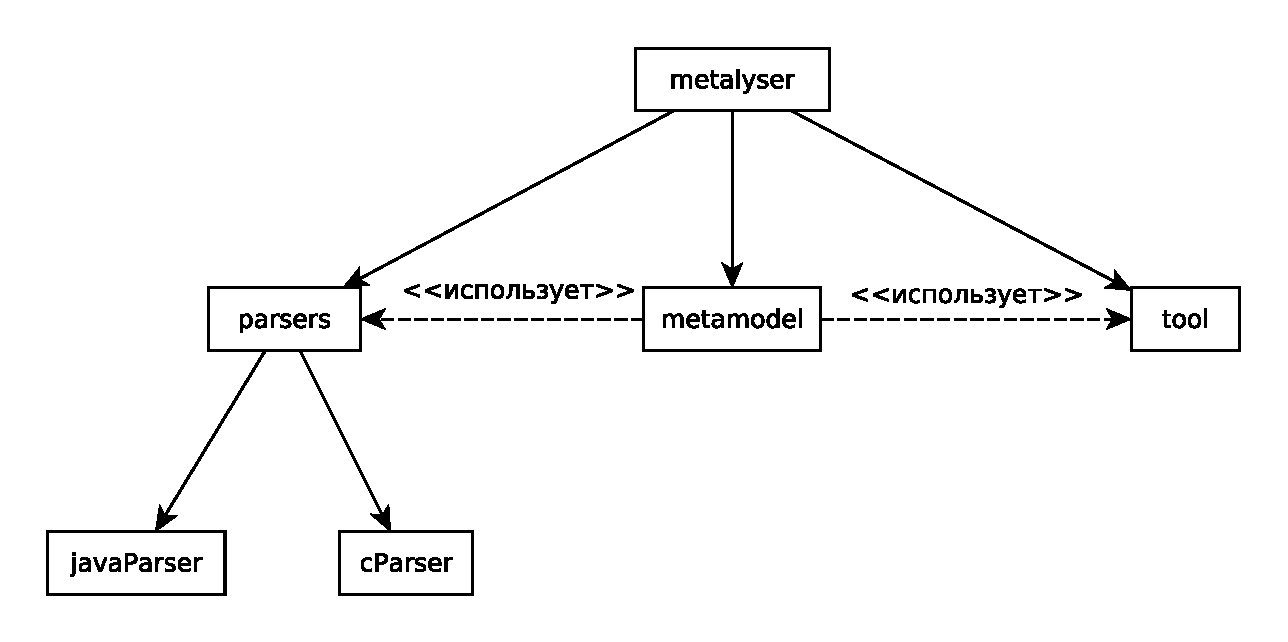
\includegraphics[width=\textwidth]{project_structure.eps}
    \end{center}
    \caption{Структура maven-проекта}
    \label{fig:project_structure}
\end{figure}

Рассмотрим подробнее приведенную структуру:

\begin{enumerate}
    \item Модуль верхнего уровня называется \texttt{metalyser} (Meta-Analyser) и
    является корнем всего проекта. В нем размещаются зависимости и плагины maven,
    необходимые для сборки всей программной системы.
    \item Модуль \texttt{parsers} является родительским модулем для
    преобразователей языка Java и C, поставляемых вместе с разработанной средой.
    \item Модуль \texttt{javaParser} является преобразователем для языка Java.
    Аналогично, модуль \texttt{cParser} используется для импортирования систем,
    написанных на языке C.
    \item Модуль \texttt{metamodel} является реализацией метамодели,
    описывающей анализируемую систему. Данный модуль реализован в виде
    библиотеки классов и не предназначен для непосредственного использования
    (он не содержит Main-класса для запуска), а используется в виде зависимости
    в остальных модулях системы.
    \item Модуль \texttt{tool} является реализацией инструментальной среды.
\end{enumerate}

%%%%%%%%%%%%%%%%%%%%%%%%%%%%%%%%%%%%%%%%%%%%%%%%%%%%%%%%%%%%%%%%%%%%%%%%%%%%%%%%
\section{Разработка метамодели}
%%%%%%%%%%%%%%%%%%%%%%%%%%%%%%%%%%%%%%%%%%%%%%%%%%%%%%%%%%%%%%%%%%%%%%%%%%%%%%%%
\subsection{Общая структура}

На основе анализа возможной архитектуры метамодели (см.
п.п.~\ref{sec:metamodel_architecture}), было принято взять за основу
архитектуру, предложенную стандартом MOF. Недостатком данной архитектуры
является ее громоздкость: полученные метамодели охватывают широкий спектр
возможных задач, что делает их достаточно объемными и сложными в использовании.
Исходя из требований к системе, было решено модифицировать исходную архитектуру,
а именно были убраны отдельные классы для отображения отношений между объектами.
Вместо этого ссылки на зависимые объекты хранятся непосредственно в самих
классах. Из-за этого теряется семантическая информация о видах отношений, но
намного сокращается количество используемых классов, что сильно упрощает
использование библиотеки.

Таким образом, полученная метамодель не является полностью MOF-совместимой, но,
если в дальнейшем развитии проекта будет необходима такая совместимость для
взаимодействия со сторонними приложениями, не составит труда привести ее к
полной совместимости.

Принимая во внимание все перечисленные замечания, была разработана
соответствующая структура метамодели (краткая UML-диаграмма классов приведена на
рис.~\ref{fig:metamodel_uml}). Стоит отметить, что на данной диаграмме, для
уменьшения ее размеров, были опущены все методы, отношения между классами и
некоторые наследники основных суперклассов.

\begin{sidewaysfigure}[!htbp]
    \begin{center}
        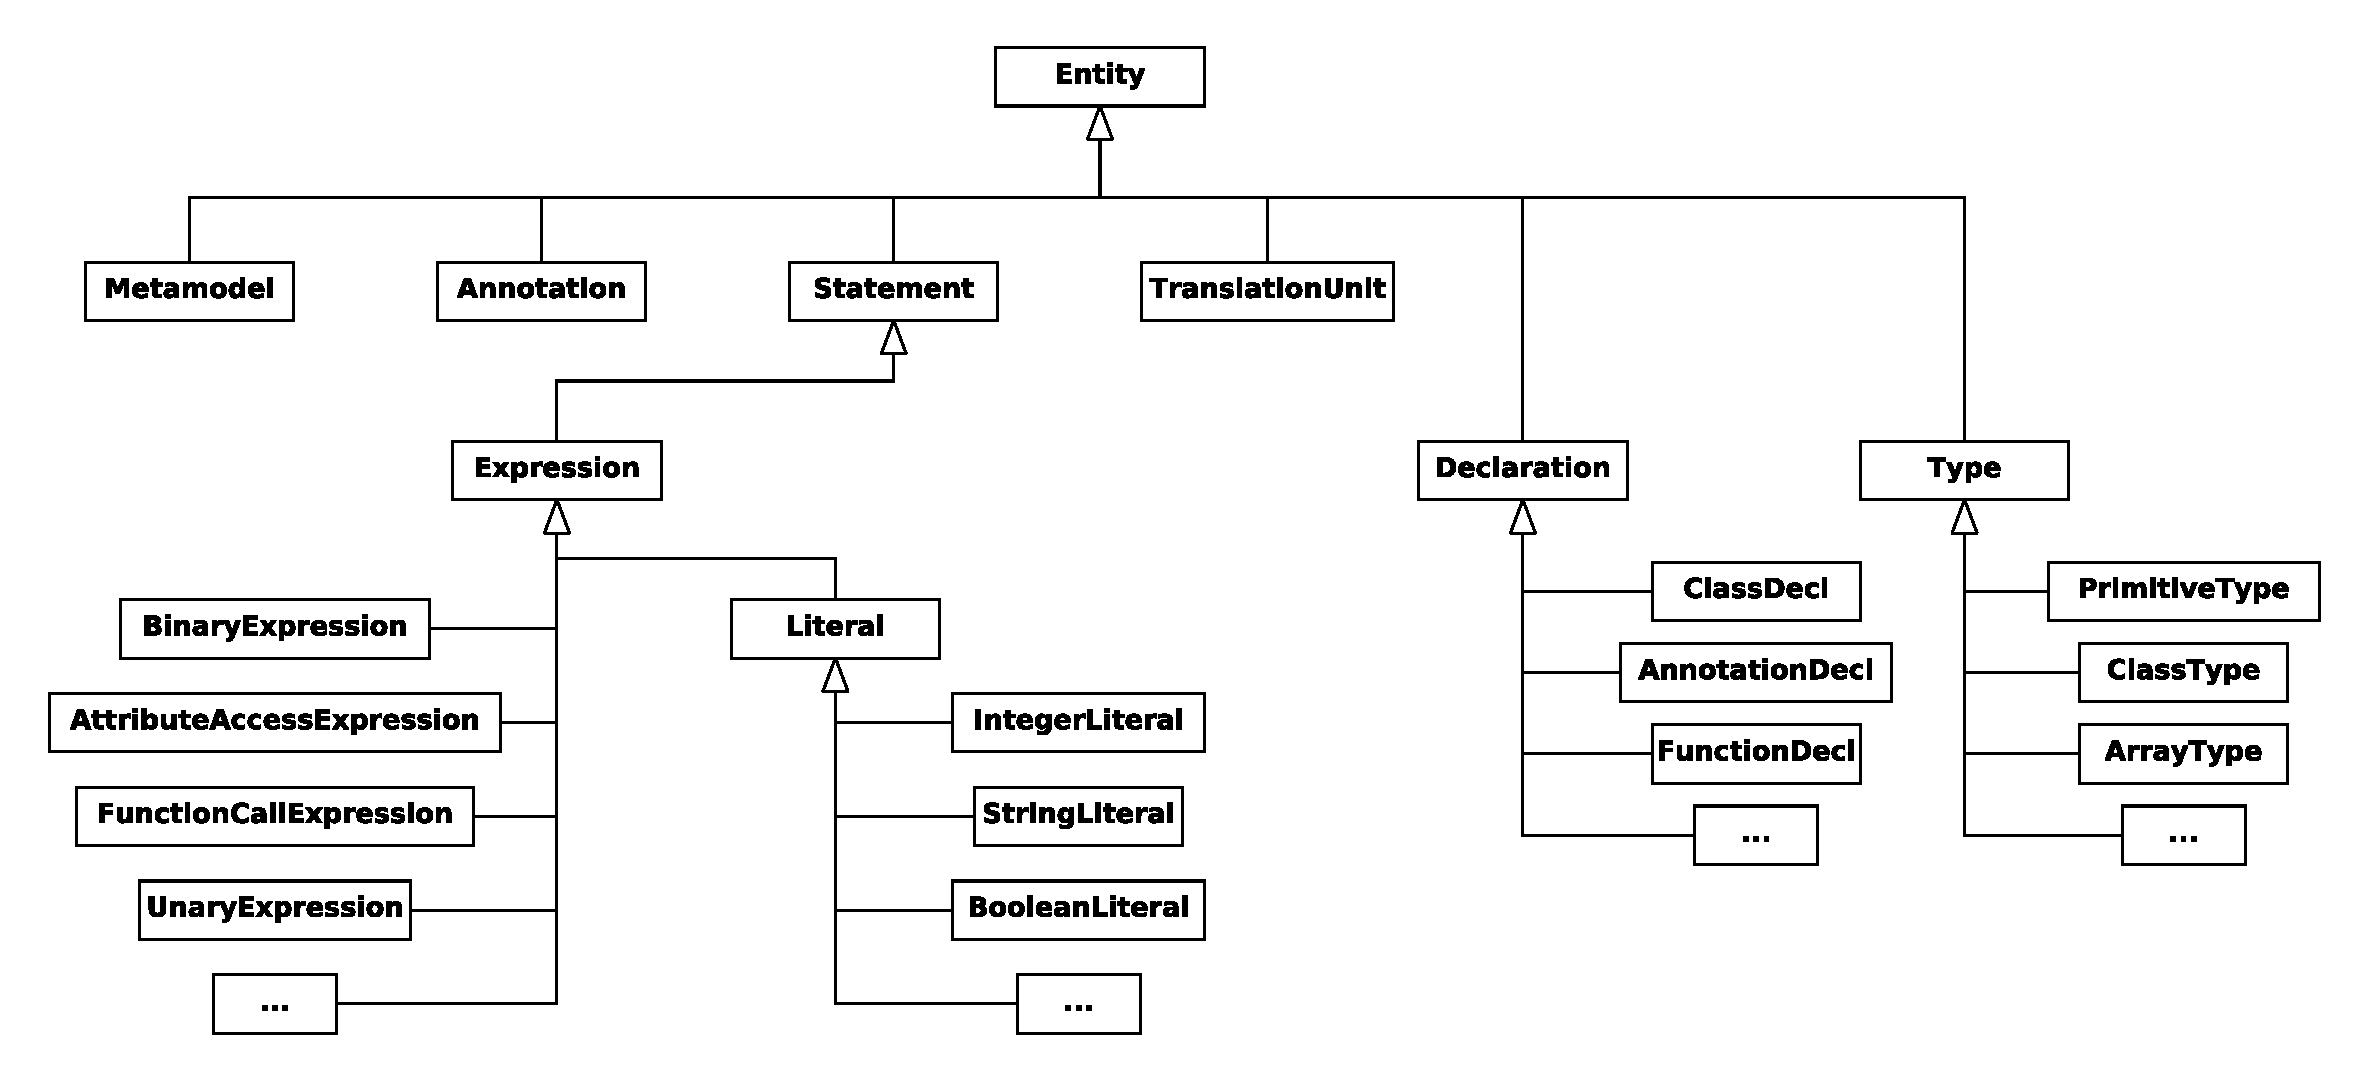
\includegraphics[width=\textwidth]{metamodel_uml.eps}
    \end{center}
    \caption{Упрощенная диаграмма классов метамодели}
    \label{fig:metamodel_uml}
\end{sidewaysfigure}

Рассмотрим подробнее некоторые из классов:

\subsubsection{Entity}

\begin{lstlisting}[caption={Интерфейс Entity}]
public interface Entity {
    public void accept(final Visitor visitor);
}
\end{lstlisting}

От интерфейса \texttt{Entity} наследуются все классы метамодели. Класс содержит
лишь один метод - \texttt{accept}, который необходим для обхода дерева, которое
представляет из себя построенная модель. Таким образом для проведения анализа
метамодели был реализован паттерн ``Посетитель'' (подробнее про обход
дерева объектов описано в п.п.~\ref{subsec:metamodel_operations}).

\newpage
\subsubsection{Metamodel}

\begin{lstlisting}[caption={Класс Metamodel}]
public class Metamodel implements Entity {
    private final List<TranslationUnit> units;

    ...
}
\end{lstlisting}

Данный класс является контейнером верхнего уровня для объектов типа
\texttt{TranslationUnit}. Он предназначен для сборки результатов работы
преобразователей над каждым из файлов с исходным кодом анализируемой программной
системы.

\vspace{10pt}
\subsubsection{TranslationUnit}

\begin{lstlisting}[caption={Класс TranslationUnit}]
public class TranslationUnit implements Entity {
    private final List<Import> imports;
    private final List<Declaration> types;

    ...
}
\end{lstlisting}

Класс \texttt{TranslationUnit} отображает одну единицу трансляции при работе
преобразователя. Обычно ей соответствует один файл с исходным кодом (за
исключением, например, языка C, где в каждый файл на этапе работы препроцессора
вставляется текст используемых заголовочных или любых других файлов,
подключенных при помощи директивы \texttt{\#include}). Таким образом, обычно при
трансляции всей анализируемой системы в результате работы преобразователя
будет получено несколько объектов типа \texttt{TranslationUnit}, которые затем
должны быть объединены в один объект типа \texttt{Metamodel}.

\vspace{10pt}
\subsubsection{Annotation}

\begin{lstlisting}[caption={Класс Annotation}]
public class Annotation implements Entity {
    private final String name;
    private final Map<String, Entity> values;
    private final Entity value;

    ...
}
\end{lstlisting}

Данный класс предназначен для описания аннотаций (например, в языке Java) или им
подобных элементов) (например, декораторов в языке Python). Если аннотация имеет
параметры, то существует два варианта их хранения:

\begin{enumerate}
    \item Если параметров несколько, то они помещаются в контейнер
    \texttt{values}. Необходимо учитывать, что в данном случае параметры
    являются именованными.
    \item Если аннотация принимает один параметр, то он может быть неименованным
    и помещаться в поле \texttt{value}.
\end{enumerate}

\vspace{10pt}
\subsubsection{Statement}

Класс \texttt{Statement} является базовым для всех выражений в исходном коде
программы. Примером наследников являются классы \texttt{IfStatement} (ветвление
вида ``if-else'') и \texttt{WhileStatement} (цикл ``while'').

\subsubsection{Expression}

\begin{lstlisting}[caption={Класс Expression}]
public abstract class Expression implements Statement {
    protected final Type type;

    ...
}
\end{lstlisting}

Данный класс по своему назначению аналогичен классу \texttt{Statement}, но, в
отличие от него, предназначен для описания выражений, имеющих тип. Примером
таких выражений может быть обращение к переменной (класс
\texttt{VariableReferenceExpression}), арифметические выражения (классы
\texttt{BinaryExpression} и \texttt{UnaryExpression}), вызов функции (класс
\texttt{FunctionCallExpression}) и т.д. Следует отметить, что типизированные
выражения также являются обычными выражениями и могут использоваться аналогично
другим наследникам класса \texttt{Statement}.

\vspace{10pt}
\subsubsection{Type}

Данный класс предназначен для описания различного вида типов, как примитивных,
так и пользовательских. Наследниками этого класса являются, например, классы
\texttt{PrimitiveType} (примитивные типы) и \texttt{ArrayType} (массивы).

\subsubsection{Literal}

Класс \texttt{Literal} отображает различного вида литералы в исходном коде
программы. Примерами литералов могут являться целочисленные литералы (1, 42, 88),
строковые литералы (``foo'', ``barbaz'') и т.д.

\subsubsection{Declaration}

\begin{lstlisting}[caption={Класс Declaration}]
public abstract class Declaration implements Entity {
    protected final String name;
    protected Visibility visibility;
    protected final List<String> modifiers;
    protected final List<Annotation> annotations;

    ...
}
\end{lstlisting}

Класс \texttt{Declaration} является суперклассом для объявлений типов и
глобальных переменных. Каждое объявление может быть помечено аннотациями
(\texttt{annotations}) или различными модификаторами (например, \texttt{final} в
языке Java или \texttt{const} в С). Один вид модификаторов, а именно
модификаторы доступа, вынесены в тип \texttt{Visibility}. Это сделано для
облегчения подсчета некоторых видов метрик, а также потому что в большинстве
языков программирования назначение этих модификаторов совпадает (поэтому данное
допущение не ударит по универсальности метамодели). Примерами наследников
данного класса являются классы \texttt{ClassDecl} (объявление класса) и
\texttt{FunctionDecl} (объявление функции).

\vspace{10pt}
\subsection{Проведение операций над метамоделью}
\label{subsec:metamodel_operations}

Существует два подхода к реализации паттерна ``Посетитель'' в языке
Java:

\begin{enumerate}
    \item ``Классический'' подход
    \item Подход с использованием рефлексии в языке Java (Java Reflection
    API~\cite{Gosling2013})
\end{enumerate}

Рассмотрим оба варианта подробнее:

\subsubsection{``Классический'' подход}

В данном случае в классе-``посетителе'' необходимо реализовывать методы
\texttt{visit} для каждого типа иерархии объектов. К недостаткам данного подхода
можно отнести очень малую гибкость - при изменении иерархии классов, над
которой совершается обход, аналогичные изменения необходимо вносить в каждый
из классов-``посетителей''.

\subsubsection{Подход с использованием рефлексии}

Подход с использованием рефлексии использует метод языка Java
\texttt{Java.lang.Class.getMethod()} для поиска метода \texttt{visit} для
типа объекта-параметра. Достоинствами данного метода является отсутствие
необходимости реализации метода \texttt{visit} для каждого возможного класса из
иерархии: пользователь должен реализовать метод только для тех классов, которые
необходимы для той или иной процедуры, производимой над этой иерархией.
Недостатком данного подхода является пониженное быстродействие по сравнению в
``классическим'' подходом (из-за низкой производительности Reflection API).

Так как метамодель, в соответствии с требованиями, должна быть расширяемой и
позволять легко добавлять новые классы к уже существующим, то было принято
решение использовать подход с использованием рефлексии.

Исходя из вышесказанного был разработан интерфейс \texttt{Visitor}:

\begin{lstlisting}[caption={Базовый класс для обхода метамодели}]
public interface Visitor {
    public void dispatch(final Entity entity);
    public void navigate(final Entity entity);
}
\end{lstlisting}

Метод \texttt{dispatch} вызывается на корневом объекте метамодели (чаще всего
это экземпляр класса \texttt{Metamodel}, но это условие не является
обязательным) и инициирует процедуру обхода. Метод \texttt{navigate}
предназначен для определения порядка обхода вложенных элементов метамодели: для
каждого класса, унаследованного от \texttt{Entity}, необходимо переопределить
метод \texttt{accept}, в котором пользователь может задавать, в каком порядке
будут посещены поля этого класса. Также поддерживается навигация
непосредственно из класса, реализующего интерфейс \texttt{Visitor}: для
необходимо переопределить метод \texttt{navigate}, чтобы он оставался пустым.

Примером реализации интерфейса \texttt{Visitor} является класс
\texttt{VisitorAdapter}:

\begin{lstlisting}[caption={Реализация интерфейса Visitor}]
public class VisitorAdapter implements Visitor {
    @Override
    public void dispatch(final Entity entity) {
        if (entity == null) return;
        try {
            final Method m = getClass().getMethod("visit",
                new Class<?>[] { entity.getClass() });
            m.invoke(this, new Object[] { entity });
        } catch (NoSuchMethodException ex) {
            // логгирование ошибки
        } catch (IllegalAccessException | IllegalArgumentException | InvocationTargetException ex) {
            // логгирование ошибки
        }
        navigate(entity);
    }

    @Override
    public void navigate(Entity entity) {
        entity.accept(this);
    }
}
\end{lstlisting}

Переопределенный метод \texttt{dispatch} работает следующим образом:

\begin{enumerate}
    \item Получение метода \texttt{visit} для класса объекта, переданного
    в качестве параметра.
    \item В случае отсутствия такого метода, происходит запись сообщения с
    соответствующей информацией в лог, но ход программы не прерывается.
    \item Вызов метода на объекте-параметре.
    \item Вызов метода \texttt{navigate} для дальнейшего обхода объектов
    метамодели. В данном случае используется навигация по-умолчанию, описанная
    в классах метамодели.
\end{enumerate}

\subsection{Выбор фреймворка для сериализации}

Для языка Java существует множество фреймворков для генерации XML-файлов,
самыми популярными из них являются:

\nomenclature{JAXB}{Java Architecture for XML Binding, фреймворк для
XML-сериализации для языка Java}
\nomenclature{Simple}{фреймворк для XML-сериализации для языка Java}
\nomenclature{XStream}{фреймворк для XML-сериализации для языка Java}
\nomenclature{XMLBeans}{фреймворк для XML-сериализации для языка Java}

\begin{enumerate}
    \item Java Architecture for XML Binding (JAXB)
    \item Simple
    \item XStream
    \item XMLBeans
 \end{enumerate}

Во всех фреймворках, кроме XMLBeans, описание правил сериализации производится
при помощи аннотирования необходимых элементов классов.

\subsubsection{JAXB}

JAXB представляет собой стандарт, описывающий преобразование Java объектов в XML
(маршалинг) и обратно (демаршалинг). Так как JAXB является стандартом, то
существует несколько его реализаций, например, Metro, EclipseLink MOXy, JaxMe.
Отличительной особенностью данного стандарта является наличие его реализации в
составе Java SE начиная с  версии 6, тем самым исключается необходимость
внедрения дополнительных зависимостей в проект.

Пример использования аннотаций JAXB:

\begin{lstlisting}[caption={Пример использования фреймворка JAXB}]
@XmlRootElement
public class Customer {
    String name;
    int age;
    int id;

    @XmlElement
    public void setName(String name) {
        this.name = name;
    }

    @XmlElement
    public void setAge(int age) {
        this.age = age;
    }

    @XmlAttribute
    public void setId(int id) {
        this.id = id;
    }

    ...
}
\end{lstlisting}

XML-файл после сериализации:

\begin{lstlisting}[language=xml, caption={Полученный XML-файл}]
<?xml version="1.0" encoding="UTF-8" standalone="yes"?>
<customer id="100">
    <age>23</age>
    <name>Alexander</name>
</customer>
\end{lstlisting}

\subsubsection{Simple}

Фреймворк Simple организован таким образом, чтобы как можно больше снизить
необходимость конфигурирования, что уменьшает количество используемых аннотаций
в коде. Еще одной отличительной особенностью данного фреймворка является наличие
возможности десереализации неизменяемых объектов, что актуально для большинства
классов разработанной метамодели.

Пример использования:

\begin{lstlisting}[caption={Пример использования фреймворка Simple}]
@Root
public class Example {
   @Element
   private String text;

   @Attribute
   private int index;

   ...
}
\end{lstlisting}

Полученный XML-файл:

\begin{lstlisting}[language=xml, caption={Полученный XML-файл}]
<example index="123">
   <text>Example message</text>
</example>
\end{lstlisting}

\subsubsection{XStream}

XStream по своим возможностям практически ничем не отличается от уже описанной
раннее реализации JAXB. К недостаткам данного фреймворка можно отнести
отсутствие подробной документации.

Пример использования:

\begin{lstlisting}[caption={Пример использования фреймворка XStream}]
@XStreamAlias("message")
class RendezvousMessage {

    @XStreamAlias("type")
    @XStreamAsAttribute
    private int messageType;

    @XStreamImplicit(itemFieldName="part")
    private List<String> content;

    ...
}
\end{lstlisting}

Полученный XML-файл:

\begin{lstlisting}[language=xml, caption={Полученный XML-файл}]
<message type="15">
    <part>firstPart</part>
    <part>secondPart</part>
</message>
\end{lstlisting}

\subsubsection{XMLBeans}

\nomenclature{XSD}{XML Schema Definition, язык описания схем XML}

Фреймворк XMLBeans является часть проекта Apache XML. В отличие от всех
остальных фреймворков, XMLBeans создает Java-классы на основе схем, описанных на
языке XSD (XML Schema Definition), что делает его непригодным к использованию
в разрабатываемом проекте.

Таким образом, после проведения анализа, для сериализации метамодели был выбран
фреймворк Simple. Ключевым фактором является возможность данного фреймворка
сериализовывать неизменяемые объекты, а наличие сторонней зависимости не
является проблемой, благодаря системе сборки Maven.

Пример использования фреймворка Simple в разработанной метамодели:

\begin{lstlisting}[caption={Пример использования фреймворка Simple в метамодели}]
public abstract class Declaration implements Entity {
    @Element(required = false)
    protected final String name;
    @Element
    protected Visibility visibility;
    @ElementList(required = false)
    protected final List<String> modifiers;
    @ElementList(required = false)
    protected final List<Annotation> annotations;

    public Declaration(
        @Element(name = "name")
        final String name,
        @Element(name = "visibility")
        final Visibility visibility,
        @ElementList(name = "modifiers")
        final List<String> modifiers,
        @ElementList(name = "annotations")
        final List<Annotation> annotations) {

        ...
    }

    ...
}
\end{lstlisting}

Аннотация \texttt{@Element} обозначает один тэг в итоговом XML-документе, где
аргумент \texttt{required} указывает на то, что данный тэг не является
обязательным. Аннотация \texttt{@ElementList} описывает коллекцию тэгов. Так как
класс \texttt{Declaration} является неизменяемым, то для десереализации
необходимо предоставить конструктор, позволяющий инициировать все поля класса,
при этом каждый параметр необходимо пометить соответствующей аннотаций с
указанием имени поля.

В данном проекте используется версия Simple 2.7.1, выпущенная в 2013 году.

Пример сериализованной метамодели приведен в приложении~\ref{sec:metamodel_xml}.

%%%%%%%%%%%%%%%%%%%%%%%%%%%%%%%%%%%%%%%%%%%%%%%%%%%%%%%%%%%%%%%%%%%%%%%%%%%%%%%%
\section{Разработка преобразователей}
%%%%%%%%%%%%%%%%%%%%%%%%%%%%%%%%%%%%%%%%%%%%%%%%%%%%%%%%%%%%%%%%%%%%%%%%%%%%%%%%

При разработке архитектуры преобразователей
(п.п.\ref{sec:transformer_architerture}) было принято решение об использовании
генераторов парсеров для проведения лексического и синтаксического анализа при
построении модели анализируемой программы.

\subsection{Выбор генератора лексического и синтаксического анализаторов}

Наиболее популярными генераторами парсеров (которые активно разрабатываются и
поддерживатся) на языке Java на данный момент являются следующие программные
средства:

\nomenclature{ANTLR}{ANother Tool for Language Recognition, инструмент для
генерации лексических и синтаксических анализаторов}
\nomenclature{JavaCC}{Java Compiler Compiler, генератор синтаксических
анализаторов}
\nomenclature{Jparsec}{генератор синтаксических и лексических анализаторов}

\begin{itemize}
    \item ANTLR (ANother Tool for Language Recognition)
    \item JavaCC (Java Compiler Compiler)
    \item Jparsec
\end{itemize}

\subsubsection{ANTLR}

ANother Tool for Language Recognition - генератор синтаксических и лексических
анализаторов. Данное средство генерирует нисходящий анализатор на основе LL(*)
грамматики. Достоинствами данного генератора является комбинированная грамматика
(единая для парсера и лексера), наличие среды разработки (ANTLRWorks), подробная
диагностика ошибок, а так же способность разбирать леворекурсивные грамматики
(которые обычно недопустимы при построении LL-анализаторов)~\cite{parr_definitive_2007}.

Для описания грамматики используется форма, близкая к РБНФ:

\begin{lstlisting}[caption={Пример грамматики, используемой в средстве ANTLR}]
 grammar T; //имя грамматики
//нетерминальные символы:
msg : 'name' ID ';'
    {
        System.out.println("Hello, " + $ID.text + "!");
    } ;
//терминальные символы
ID: 'a'..'z' + ;//произвольное (но >=1) количество букв
WS: (' ' |'\n' |'\r' )+; // пробел, перенос строки, табуляция
\end{lstlisting}

\subsubsection{JavaCC}

Как и средство ANTLR, JavaCC генерирует парсер на основе рекурсивного спуска, но
с использованием LL(1) грамматики, что увеличивает производительность
сгенерированного кода, но также увеличивает сложность написания грамматики.

Пример грамматики:

\begin{lstlisting}[caption={Пример грамматики, используемой в средстве JavaCC}]
SKIP:  { " " | "\t" | "\n" | "\r"                    }
TOKEN: { "(" | ")" | "+" | "*" | <NUM: (["0"-"9"])+> }

void S(): {} { E() <EOF>           }
void E(): {} { T() ("+" T())*      }
void T(): {} { F() ("*" F())*      }
void F(): {} { <NUM> | "(" E() ")" }
\end{lstlisting}

\subsubsection{Jparsec}

Jparsec так же используется для генерации парсера на основе рекурсивного спуска.
Главной отличительной особенностью данного генератора является тот факт, что он
использует комбинаторы синтаксического анализа. Это значит, что он не использует
отдельный файл с грамматикой в форме РБНФ, на основе которого генерируется код
парсера на языке Java. Вместо этого каждому нетерминальному символу грамматики
ставится в соответствие объект языка Java, а операции по составлению данного
символа - альтернатива (символ ``|'' в РБНФ), зависимость (последовательность
лексем) и т.д., описываются при помощи методов этого объекта.

Приведем пример парсера, использующего данный фреймворк:

\begin{lstlisting}[caption={Пример парсера, использующего фреймворк Jparsec}]
private static final Terminals OPERATORS =
    Terminals.operators("+", "-", "*", "/", "(", ")");

static final Parser<?> TOKENIZER =
    Parsers.or(Terminals.DecimalLiteral.TOKENIZER,
               OPERATORS.tokenizer());

static Parser<?> term(String... names) {
    return OPERATORS.token(names);
}

static final Parser<BinaryOperator> WHITESPACE_MUL =
    term("+", "-", "*", "/").not().retn(BinaryOperator.MUL);

static <T> Parser<T> op(String name, T value) {
    return term(name).retn(value);
}

static Parser<Double> calculator(Parser<Double> atom) {
    Parser.Reference<Double> ref = Parser.newReference();
    Parser<Double> unit =
        ref.lazy().between(term("("), term(")")).or(atom);
    Parser<Double> parser = new OperatorTable<Double>()
        .infixl(op("+", BinaryOperator.PLUS), 10)
        .infixl(op("-", BinaryOperator.MINUS), 10)
        .infixl(op("*", BinaryOperator.MUL).or(WHITESPACE_MUL), 20)
        .infixl(op("/", BinaryOperator.DIV), 20)
        .prefix(op("-", UnaryOperator.NEG), 30)
        .build(unit);
    ref.set(parser);
    return parser;
}
\end{lstlisting}

Использование данного подхода исключает необходимость фазы генерации кода при
сборке проекта, а разработанный код в несколько раз меньше по объему, чем
сгенерированный. К недостаткам данного фреймворка можно отнести сложную
реализацию необходимой грамматики и неудовлетворительное информирование об
ошибках при проведении разбора.

Таким образом, самым совершенным средством для разработки синтаксических и
лексических анализаторов является фреймворк ANTLR, в силу простоты использования
и неплохой эффективности полученных анализаторов.

В данном проекте используется версия ANTLR 4.2.2, выпущенная в 2014 году.

\subsection{Правила использования генератора парсеров ANTLR}

Общая структура файла для описания грамматики ANTLR выглядит следующим образом:

\begin{lstlisting}[caption={Структура грамматики ANTLR}]
grammar Name; // имя грамматики
options {...}
import ... ;
tokens {...}
@actionName {...}

rule1 // правила грамматики
...
ruleN
\end{lstlisting}

Секция \texttt{import} предназначена для импортирования других файлов с
правилами грамматики, тем самым позволяя создавать иерархичную структуру
ANTLR-проекта.

Секция \texttt{tokens} позволяет явно задавать типы лексем лексического
анализатора. На практике это означает, что будет сгенерировано перечисление
(enum), которое затем может быть использовано в коде парсера для отсылке к той
или иной лексеме.

Правила вида \texttt{@действие {...}} позволяют использовать набор определенных
действий, поддерживаемых ANTLR. Примерами являются действие \texttt{@header} для
описания заголовочной части сгенерированного кода парсера и действие
\texttt{@after} для генерации кода, который будет выполнен непосредственно перед
вызовом определенного правила грамматики. Пример использования приведен в
листинге~\ref{lst:actions}:

\begin{lstlisting}[caption={Использование действий ANTLR}, label={lst:actions}]
grammar Count;
// объявление пакета, в котором располагается код парсера
@header {
package foo;
}

@members {
int count = 0; // объявление члена класса парсера
}

list
// вывод количества чисел во входной последовательности лексем
@after {System.out.println(count + " ints");}
 : INT {count++;} (',' INT {count++;} )*
 ;

INT : [0-9]+ ;
\end{lstlisting}

Секция \texttt{options} задает параметры генерации кода, например, язык на
котором будет сгенерирован полученный парсер.

ANTLR позволяет создавать смешанные грамматики, т.е. в одном и том же файле
задаются как правила синтаксического анализа, так и лексического. Правила
разбора лексем имеют вид \texttt{ИМЯ : правило}, где правая часть задает
название правила, а левая - правило его разбора. Аналогичный формат имеют
правила для нетерминальных символов с той лишь разницей, что имена лексем
задаются заглавными буквами, а нетерминалов - прописными.

\subsubsection
